\documentclass[a4paper,12pt]{article}
\usepackage[utf8]{vietnam}
\usepackage{graphicx}
\usepackage{geometry}
\usepackage{tikz}
\usetikzlibrary{calc}
\usepackage{xcolor}
\usepackage{enumitem}
\usepackage{titlesec}
\usepackage{helvet}
\renewcommand{\familydefault}{\sfdefault}
\geometry{margin=2.5cm}

\begin{document}
\fontsize{14pt}{16pt}\selectfont
%_______Trang bìa________
\begin{titlepage}
\begin{center}
 
\begin{tikzpicture}[remember picture, overlay]
  \draw[line width=0.5pt] 
    ($ (current page.north west) + (1.5cm,-1.5cm) $) rectangle 
    ($ (current page.south east) + (-1.5cm,1.5cm) $);
\end{tikzpicture}

\vspace*{0.5cm}
\textbf{POSTS AND TELECOMMUNICATIONS INSTITUTE OF TECHNOLOGY}\\[0.2cm]
\textbf{FACULTY OF INFORMATION TECHNOLOGY 1}\\[1.5cm]

\includegraphics[width=0.15\textwidth]{ptit-logo.png}\\[3cm]

\textbf{\Large PYTHON PROGRAMMING}\\[0.5cm]
\textbf{ASSIGNMENT 1}\\[0.5cm]
\textbf{\LARGE FOOTBALL DATA ANALYSIS}\\[3cm]

{\Large
\begin{center}
\begin{tabular}{r@{: }l}
\textbf{Instructor} & Kim Ngoc Bach \\
\textbf{Student} & Pham Lan Anh \\
\textbf{Student ID} & B23DCCE010 \\
\textbf{Class ID} & D23CQCE04-B \\
\end{tabular}
\end{center}
}

\vfill
\textit{Hanoi}

\end{center}
\end{titlepage}

\newpage
%_______Mục lục________
\begin{center}
    \textcolor{blue}{\textbf{\Large TABLE OF CONTENTS}}
\end{center}

\begin{enumerate}[label=\textbf{\arabic*.}, leftmargin=1.5cm]
    \item \textbf{INTRODUCTION}
    \item \textbf{COLLECTING STATISTICAL DATA OF PREMIER LEAGUE FOOTBALL PLAYERS}
    \item \textbf{DATA ANALYSIS}
    \begin{enumerate}[label=\arabic{enumi}.\arabic*.]
        \item Identify the top 3 and bottom 3 players in each statistical category
        \item Find the median, mean, and standard deviation
        \item Draw histograms to show the distribution of each statistic
        \item Determine the player with the highest overall score
    \end{enumerate}
    \item \textbf{PLOT 2D VISUALIZATION OF STATISTICAL DATA}
    \item \textbf{CONCLUSION}
\end{enumerate}

\newpage
%_______Giới thiệu________
\section*{\textcolor{blue}{\Large 1. Introduction}}

\setlength{\parindent}{0pt}  
\setlength{\parskip}{1em} 
In recent years, data analysis has played an increasingly important role in professional sports, especially football. Statistical data is now widely used by clubs, analysts, and fans to assess player performance, optimize team strategies, and inform financial decisions such as player transfers. This project aims to utilize the Python programming language to collect, process, and analyze football player statistics from the 2024--2025 English Premier League season.

The primary goal of this project is to develop a system that collects a wide range of player performance metrics from public data sources. These indicators include playing time, goals, assists, expected goals (xG), defensive actions, passing statistics, and more. Only players with more than 90 minutes of playtime are included in the dataset, which is sourced from \textit{fbref.com}, a well-known football statistics website. The collected data is stored in a file named \texttt{results.csv}.

The second objective is to perform statistical analysis on the data. This includes identifying top-performing players, computing summary statistics such as mean, median, and standard deviation, and visualizing data distributions using histograms. Additionally, the project aims to determine which group of players performs best based on aggregated metrics.

Furthermore, clustering techniques are applied using the K-Means algorithm, in combination with Principal Component Analysis (PCA), to reduce dimensionality and group players based on similar performance characteristics. The clustering results are visualized on a 2D plot for easy interpretation and analysis.

Finally, the project collects player market values from \textit{footballtransfers.com} and proposes a machine learning approach (using Random Forest Regression) to estimate player market value based on in-game statistics. This involves preprocessing, feature selection, model training, and evaluation using metrics such as Mean Squared Error (MSE).

Through this project, the author not only enhances practical skills in Python-based data science but also gains a deeper understanding of how statistical methods and machine learning algorithms can be applied in real-world sports analytics, laying the foundation for broader future applications.

\newpage
%_______Bài 1________
\section*{\textcolor{blue}{\Large 2. Collecting statistical data of premier league football players}}
The data is collected from the following web pages of the FBRef website:
\begin{itemize}
    \item \texttt{stats\_standard\_9}: General player statistics
    \item \texttt{stats\_keeper\_9}: Goalkeeper statistics
    \item \texttt{stats\_shooting\_9}: Shooting statistics
    \item \texttt{stats\_passing\_9}: Passing statistics
    \item \texttt{stats\_gca\_9}: Goal Creation Actions (GCA) statistics
    \item \texttt{stats\_defense\_9}: Defensive statistics
    \item \texttt{stats\_possession\_9}: Possession statistics
    \item \texttt{stats\_misc\_9}: Miscellaneous statistics
\end{itemize}

\titleformat{\section}
  {\bfseries\Large}
  {\thesection.}{1em}{}

\setlist[itemize]{noitemsep, topsep=0pt}

\textbf{a) Web Scraping} \\
The web scraping is performed using the Selenium library to automate a browser and extract data from HTML tables. The implementation corresponds to the following steps:
\begin{itemize}
    \item \textit{\textcolor{blue}{Send an HTTP request to the target URL using Selenium}}: the script initializes a headless Chrome browser via the \texttt{init\_driver()} function and navigates to the target URL with \texttt{driver.get(url)}.
    \item \textit{\textcolor{blue}{Parse the returned HTML content using Selenium}}: the script directly accesses DOM elements via Selenium’s \texttt{find\_element()} and \texttt{find\_elements()} methods.
    \item \textit{\textcolor{blue}{Locate the relevant HTML table using a CSS Selector}}: the script uses \texttt{driver.find\_element(By.CSS\_SELECTOR, f"table\#{table\_id}")} to find the desired table, then iterates over its \texttt{<tbody>} rows to extract player data.
\end{itemize}

\vspace{1em}
\textbf{b) Extracting Table Headers} \\
The table headers are extracted from the thead section of the table. Each header corresponds to a specific statistical category for players, such as player, nationality, team, etc. The headers are filtered to only include the relevant statistics defined in the target list.

\vspace{1em}
\textbf{c) Extracting Data Rows} \\
The rows of data are extracted from the tbody section. Each row contains the statistics for a player. The values are mapped to their corresponding headers. Special handling is applied to the minutes field, converting it into an integer. Missing values are handled by inserting “N/a”.

\vspace{1em}
\textbf{d) Data Merging} \\
After scraping the data from the different stat groups, the individual DataFrames are merged into a single DataFrame.

\vspace{1em}
\textbf{e) Merge Keys} \\
The key columns used for merging the data are player and team. These two columns act as the primary identifiers across all statistical groups. The merging process is implemented sequentially using the \texttt{merge()} function provided by the pandas library.

\vspace{1em}
\textbf{f) Merging Process} \\
For each statistical group (excluding the \texttt{stats\_standard} group, which serves as the base), the script selects the relevant columns for merging. Any columns that are already present in the base DataFrame are excluded to avoid duplication, while new columns are added. The merging operation is performed using a left join, ensuring that all rows from the base dataset (i.e., all players) are retained, even if corresponding data in other stat groups is missing.

\vspace{1em}
\textbf{g) Cleaning the Data} \\
After merging, the following cleaning steps are performed:
\begin{itemize}
    \item Missing values are filled with “N/a”.
    \item Players who have played less than 90 minutes are filtered out.
    \item The columns are reordered according to the target list.
\end{itemize}

\vspace{1em}
\textbf{h) Final Output} \\
The final cleaned and merged DataFrame is sorted by the player column to ensure consistent ordering of the dataset. Column names are then renamed using a predefined mapping dictionary named \texttt{target\_name\_dict}. Finally, the complete dataset is exported and saved as a CSV file with the filename \texttt{results.csv}.

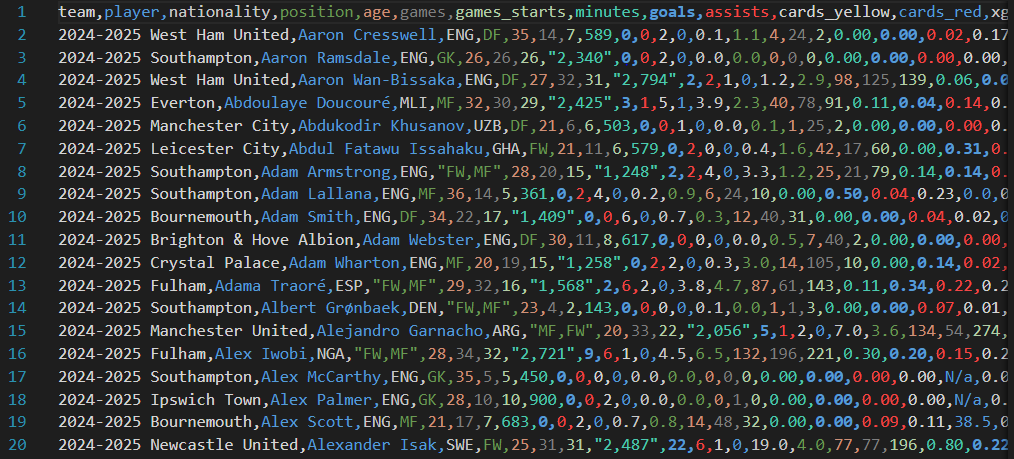
\includegraphics[width=1\textwidth]{results.PNG}

\newpage
%_______Bài 2________
\section*{\textcolor{blue}{\Large 3. Data analysis}}
\subsection*{\textbf{\Large 3.1. Identify the top 3 and bottom 3 players in each statistical category}}
This section presents the methodology and results from the analysis of a player statistical dataset. The goal is to determine individual and team performance through descriptive statistics, rankings, and data visualization.

\titleformat{\section}
  {\bfseries\Large}
  {\thesection.}{1em}{}

\setlist[itemize]{noitemsep, topsep=0pt}

\textbf{a) Loading the Data} \\
The script starts by importing the necessary libraries: pandas for data manipulation, numpy for numerical operations, and matplotlib.pyplot for plotting.
The dataset is then loaded from a file named \texttt{results.csv} using \texttt{pandas}. This dataset contains various statistics for football players, with rows representing players and columns representing different performance metrics and metadata (e.g., name, team, nationality).

\textbf{b) Converting Columns to Numeric} \\
All non-numeric entries, marked as “N/a”, are converted to “NaN” to enable accurate statistical calculations. The analysis focuses only on columns with numeric values, eliminating identifying information such as player name, nationality, and team. To ensure statistical calculations can be performed, convert all relevant columns to numeric data types.

\textbf{c) Finding Top and Bottom Performers} \\
This section describes the method used to determine the top 3 and bottom 3 players for each statistical metric. The process is implemented using pandas DataFrame functionalities and involves the following steps:
\begin{itemize}
    \item \textit{\textcolor{blue}{Eliminate Missing Values (NaN)}}: Each column is checked for missing values. If a column consists entirely of \texttt{NaN} values, it is excluded from the analysis to prevent misleading or biased results. For columns with partial missing data, rows with \texttt{NaN} values are temporarily excluded during sorting.
    \item \textit{\textcolor{blue}{Sort Data in Descending Order}}: For each statistical column, the data is sorted from high to low. This allows identification of the top 3 players with the highest values—representing the best performers for that metric.
    \item \textit{\textcolor{blue}{Sort Data in Ascending Order}}: Similarly, the column is sorted from low to high to identify the 3 players with the lowest values, representing the least effective performers in that category.
    \item \textit{\textcolor{blue}{Extract Top 3 Players}}: After sorting, the top (or bottom) 3 rows are selected using \texttt{.head(3)}.
    \item \textit{\textcolor{blue}{Format Results}}: The final output is formatted as strings to clearly show the top and bottom performers. Each entry is presented in the format \texttt{<Player>:<Value>}.
\end{itemize}

\begin{center}
    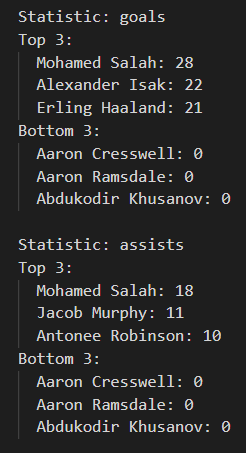
\includegraphics[width=0.5\textwidth]{top3.png}
\end{center}

\textbf{d) Conclusion} \\
This method effectively identifies the top 3 highest and lowest performing players for each statistical metric.
Insights Provided:
\begin{itemize}
    \item Player performance in each statistical category.
    \item Easy identification of standout performers.
    \item Detection of areas where players may need improvement.
\end{itemize}

Key Benefits:
\begin{itemize}
    \item Saves time compared to manual analysis.
    \item Provides quantitative insights that are objective and data-driven.
    \item Applicable to diverse sports datasets, making it a versatile tool for performance analysis.
\end{itemize}

\subsection*{\textbf{\Large 3.2. Find the median, mean, and standard deviation}}
\textbf{a) Loading the Data} \\
The analysis begins by loading a synthetic dataset containing soccer player performance statistics. This dataset is stored in a “results.csv” file and read into a pandas DataFrame.

\textbf{b) Converting Columns to Numeric} \\
All non-numeric entries, marked as “N/a”, are converted to “NaN” to enable accurate statistical calculations. The analysis focuses only on columns with numeric values, eliminating identifying information such as player name, nationality, and team. To ensure statistical calculations can be performed, convert all relevant columns to numeric data types.

\textbf{c) Calculating the Median, Mean, and Standard Deviation} \\
This section explains how to compute three essential statistical measures for each performance metric:
\begin{itemize}
    \item \textit{\textcolor{blue}{Median}}: Using the \texttt{median()} method from the pandas library to calculate the median value, which represents the middle value in a data set. It is especially valuable when the data includes outliers, as it is less affected by extreme values compared to the mean.
    \item \textit{\textcolor{blue}{Mean (Average)}}: Using the \texttt{mean()} function to calculate the mean provides an overall view of the average performance of all players, helping to determine typical performance levels.
    \item \textit{\textcolor{blue}{Standard Deviation}}: Using the \texttt{std()} function to calculate the spread of values. A high standard deviation indicates large variation in performance between players, while a low value implies consistency.
    \item \textit{\textcolor{blue}{Scope of Calculation}}: The statistics can be calculated for the entire league (to get a league-wide perspective) or for individual teams (to assess team-specific performance).
\end{itemize}

\textbf{d) Calculating Statistics for Each Team} \\
This section describes how to compute team-level statistics, which helps compare performance across different teams.

Procedure:
\begin{itemize}
    \item The data is grouped using the Team column.
    \item Numeric columns are selected for statistical analysis.
\end{itemize}

Calculate Mean and Standard Deviation:
\begin{itemize}
    \item The \texttt{<.agg()>} function is used to compute both \texttt{mean} and \texttt{std} (standard deviation) for each numeric column within each team group.
    \item The \texttt{<reset\_index()>} method ensures the result is formatted as a DataFrame with a default index.
\end{itemize}

\textbf{e) Creating the Final DataFrame} \\
This part covers organizing and saving the calculated results:
Steps:
\begin{itemize}
     \item \textit{\textcolor{blue}{Create a New DataFrame}}: A new DataFrame is created from the calculated results. It includes columns: \texttt{'Statistic'}, \texttt{'Value'}, \texttt{'Index'}, and \texttt{'Team'}.
     \item \textit{\textcolor{blue}{Save the DataFrame to CSV}}: The results are saved in a CSV file named \texttt{results2.csv} for future use or analysis. The \texttt{index=False} parameter ensures that the row index is not saved in the file. UTF-8 encoding guarantees compatibility with most systems.
\end{itemize}

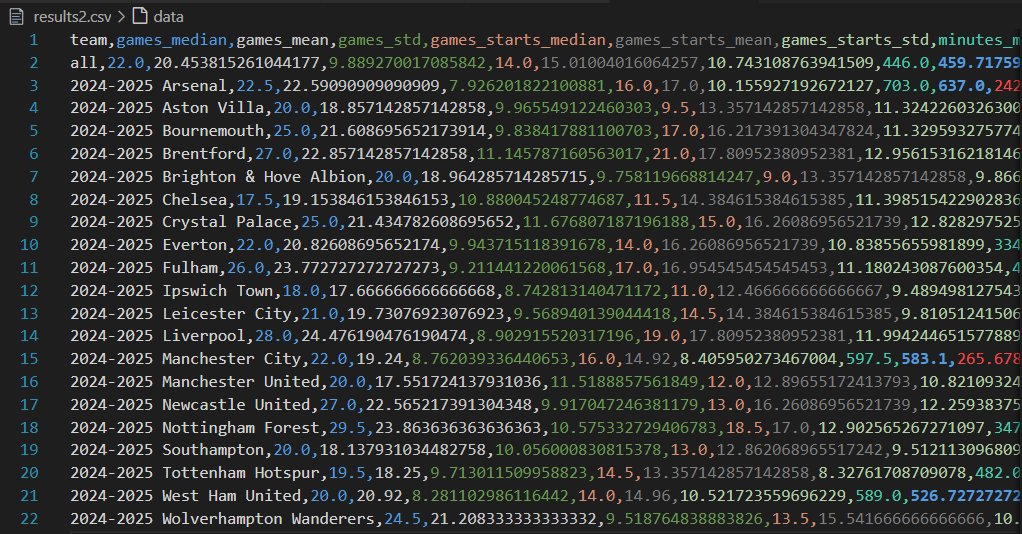
\includegraphics[width=1\textwidth]{results2.png}

\textbf{f) Conclusion} \\
This section emphasizes the purpose and value of using basic statistical indicators—\texttt{median, mean, and standard deviation}—to evaluate performance metrics in a sports dataset.
Key Takeaways:
\begin{itemize}
    \item \textit{\textcolor{blue}{Overall Performance Assessment}}: These statistics help evaluate how players and teams performed in the tournament. It gives a broad understanding of strengths and weaknesses at both individual and team levels.
    \item \textit{\textcolor{blue}{Understanding Distribution and Variation}}: By calculating standard deviation, we can observe how much variation there is in performance. This is crucial for detecting consistency vs. inconsistency across players or teams.
    \item \textit{\textcolor{blue}{Team vs. League Comparisons}}: The data enables benchmarking individual team performance against the league average. This comparative view highlights which teams are above or below average in specific metrics.
\end{itemize}
These statistical insights allow analysts to better understand player and team quality. They form a foundation for data-driven decisions, such as talent scouting, strategy planning, or identifying areas needing improvement.

\subsection*{\textbf{\Large 3.3. Draw histograms to show the distribution of each statistic}}
\textbf{a) Loading and Preparing the Data} \\
The process begins by importing player performance data from the \texttt{results.csv} file. The goal at this stage is to isolate the numeric/statistical features relevant for analysis:
\begin{itemize}
    \item Non-numeric columns like \texttt{'Player'}, \texttt{'Nation'}, \texttt{'Position'}, and \texttt{'Team'} are excluded.
    \item Only columns with actual performance metrics (e.g., goals, assists, passes) are selected for visualization.
    \item A key step here is converting all relevant columns to numeric format and replacing missing or invalid values with zeros. This ensures data consistency and all metrics can be plotted without runtime errors.
\end{itemize}

\textbf{b)  Setting Up Directories for Saving Histograms} \\
Before generating visualizations, the script organizes the output using a directory structure for clarity. A main folder named \texttt{histograms} is created. Inside it:
\begin{itemize}
    \item A \texttt{league} subfolder holds charts representing the entire dataset.
    \item A \texttt{team} sub-folder contains team-specific charts, with each team having its own subdirectory.
\end{itemize}

Purpose of this structure:
\begin{itemize}
    \item Enhances organization.
    \item Makes future retrieval and comparison of charts more intuitive.
    \item Prepares for scalability, such as adding charts for player positions or nationalities later.
\end{itemize}

\textbf{c) Plotting the Histogram for All Players} \\
Once the folders are set up, the script proceeds to generate league-wide histograms for each numeric statistic.

Process:
\begin{itemize}
    \item Loop through all numeric columns.
    \item Use \texttt{matplotlib} to create a histogram that visualizes how often different values appear in the dataset.
    \item Save the chart into the \texttt{histograms/league} folder
\end{itemize}

Purpose and Insight:
\begin{itemize}
    \item Understand overall performance trends (e.g., how many players score very high vs. very low).
    \item Spot outliers (e.g., a few players with extremely high values).
    \item Establish a performance baseline across the entire league.
\end{itemize}
This step gives a macro-level view of player statistics.

\textbf{d) Plotting Team-Specific Histograms} \\
After analyzing league-wide data, the focus shifts to individual team performance.

Process: For each team:
\begin{itemize}
    \item Filter the dataset to include only players from that team.
    \item Create a subdirectory inside \texttt{histograms/teams} using the team’s name (spaces replaced with underscores).
    \item Loop through all numeric stats and generate histograms.
    \item Save each histogram to the respective team’s folder.
\end{itemize}

Benefits of Team-Level Analysis:
\begin{itemize}
    \item Detects internal variation in team performance.
    \item Helps identify if performance is dominated by a few players or evenly distributed.
    \item Useful for comparing team structures and strategies.
\end{itemize}
For example, a team with one player scoring most of the goals will have a histogram skewed toward that player, while balanced teams will show a more uniform distribution.

\begin{center}
    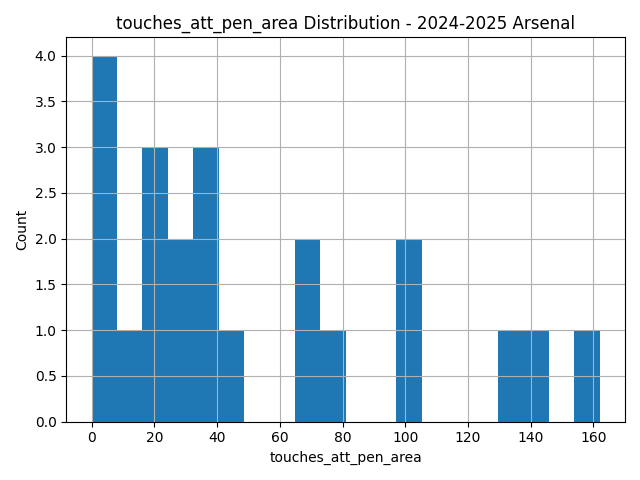
\includegraphics[width=1\textwidth]{Arsenal__att_pen.png}
\end{center}

\textbf{e) Conclusion} \\
The methodology for creating histograms allows visualization of the distribution of player statistics, both for the league and for individual teams. By creating these histograms, we can better understand the distribution of different performance metrics and draw data-driven insights about the league and teams. The histograms are stored in organized folders for easy access and further analysis.

\subsection*{\textbf{\Large 3.4. Determine the player with the highest overall score}}

\textbf{a) Aggregating Team Statistics} \\
The first step in evaluating team performance is summing all player statistics within each team:
\begin{itemize}
    \item This groups the dataset by the \texttt{Team} column.
    \item Then, it computes the total output for each statistic (e.g., total goals, total assists) across all players in that team.
    \item The result is a table showing how each team performs collectively, which forms the foundation for identifying top teams per metric.
\end{itemize}
This approach is effective for comparing overall productivity between teams.

\textbf{b) Identifying Top Teams for Each Statistic} \\
Next, the script identifies the team with the highest value for each statistic:
\begin{itemize}
    \item This loop skips any statistic that has no data and finds the team with the maximum sum for each valid statistic using \texttt{<idxmax()>}.
    \item The result is a dictionary mapping each statistic to the top-performing team for that metric.
\end{itemize}
This stage highlights specialization: some teams may dominate certain areas, such as defense or passing.

\textbf{c) Determining Overall Best-Performing Team} \\
To assess which team performs best across all statistics, the code tallies how often each team appears at the top:
\begin{itemize}
    \item This produces a ranked list showing how frequently each team led a particular stat.
    \item The team with the highest count is considered the overall best-performing team.
\end{itemize}
This technique rewards broad dominance, not just excelling in one area.

\textbf{d) Outputting Results} \\
The analysis then outputs:
\begin{itemize}
    \item The best team for each individual statistic
    \item The overall best-performing team
\end{itemize}

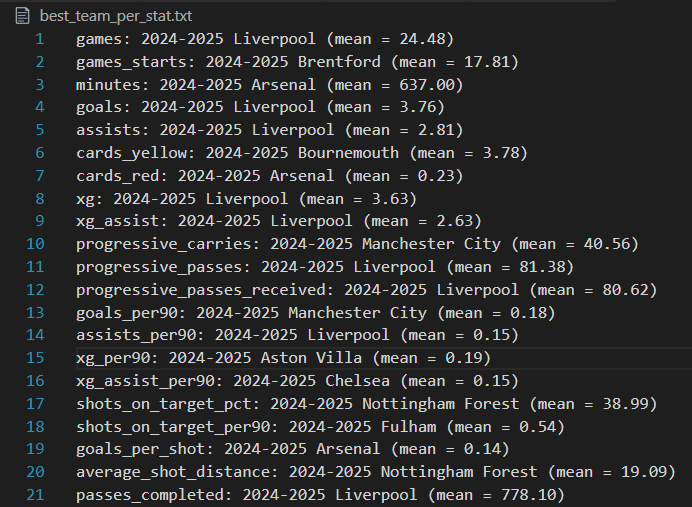
\includegraphics[width=1\textwidth]{best_team.png}

\textbf{e) Conclusion} \\
This final phase of the script provides a holistic and comparative performance analysis of teams, offering insight into:
\begin{itemize}
    \item Which teams dominate specific metrics
    \item Which team performs best overall
    \item How consistently teams perform across the board (via std and median)
\end{itemize}
By integrating sum totals, means, medians, and standard deviations, this approach offers a multi-dimensional view of team performance—ideal for scouting, strategy, and performance evaluation in professional soccer analytics.

\newpage
%_______Bài 3________
\section*{\textcolor{blue}{\Large 4. Plot 2D visualization of statistical data}}
In this section, we outline the methodology used to perform clustering on football player statistics using the K-means algorithm and visualize the resulting clusters in a two-dimensional space.

\titleformat{\section}
  {\bfseries\Large}
  {\thesection.}{1em}{}

\setlist[itemize]{noitemsep, topsep=0pt}

\textbf{a) Overview of K-means Clustering} \\
K-means clustering is an unsupervised machine learning algorithm that partitions the data into a predefined number of clusters. Each cluster is represented by its centroid, and data points are assigned to the cluster whose centroid is nearest. The K-means algorithm minimizes the within-cluster sum of squares (inertia) and iterates until convergence.

The goal of this analysis is to group players based on their performance metrics and categorize them into distinct clusters. These clusters can be visualized and labeled based on common features that are prominent within each group. In the context of football player data, the clusters typically represent different player roles such as goalkeepers, defenders, and offensive players.

\textbf{b) Preprocessing the Data} \\
Before applying the K-means clustering algorithm, several preprocessing steps are executed on the dataset:
\begin{itemize}
    \item \textit{\textcolor{blue}{Handling Non-Numeric Data}}: Columns containing non-numeric information such as player names, team names, and positions are excluded from the dataset. These fields are irrelevant for clustering since the K-means algorithm operates solely on numerical performance metrics.
    \item \textit{\textcolor{blue}{Age Conversion}}: Player age values are initially stored as strings (e.g., “25.4 years”). The script extracts the numerical component and converts it into a float, making it suitable for numerical analysis and clustering.
    \item \textit{\textcolor{blue}{Standardization}}: 
    The dataset is standardized using the \texttt{StandardScaler} from the \texttt{sklearn.preprocessing}  module. This step is crucial because K-means clustering is sensitive to the scale of input features. Standardization ensures that all features have a mean of 0 and a standard deviation of 1, which prevents any single feature from disproportionately influencing the clustering process.
\end{itemize}

\textbf{c) Determining the Optimal Number of Clusters} \\
To determine the optimal number of clusters for K-means, the script utilizes the elbow method. This approach involves calculating the inertia (sum of squared distances between data points and their nearest cluster center) for various values of \textbf{k} (the number of clusters). The optimal k is identified at the point where the rate of decrease in inertia slows down significantly, forming an "elbow" in the graph. In this analysis, the chosen value for \textbf{k} is 4.

\textbf{d) Performing K-means Clustering} \\
After identifying the optimal number of clusters (k = 4), the script applies the \textbf{K-means clustering algorithm}. The algorithm partitions the data into three clusters based on player performance metrics. Each data point is assigned to the nearest cluster based on its proximity to the cluster centroid. The assignment process is refined through multiple iterations to improve the accuracy of clustering.

\textbf{e) Labeling the Clusters} \\
Once clustering is complete, descriptive labels are assigned to each cluster to enhance interpretability. In this case, three primary player roles are used:
\begin{itemize}
    \item \textit{\textcolor{blue}{Goalkeepers}}: Players specialized in shot-saving and goal prevention.
    \item \textit{\textcolor{blue}{Defensive Players}}: Players focused on defense, including making tackles and interceptions.
    \item \textit{\textcolor{blue}{Offensive Players}}: 
    Players involved in scoring and attacking play.
\end{itemize}
The cluster centroids are analyzed by comparing key feature values to support the labeling process.

\textbf{f) Visualizing the Clusters in 2D} \\
The next step is to visualize the clusters in two dimensions to better understand the grouping of the data points. This is achieved using Principal Component Analysis (PCA), a dimensionality reduction technique that transforms the data into a lower-dimensional space while retaining as much variance as possible.
\begin{itemize}
    \item \textit{\textcolor{blue}{Data Preprocessing}}: The dataset is first loaded from a CSV file \texttt{results.csv}. Only numeric columns are selected for clustering, and any rows containing missing values are removed to ensure data integrity. The data is then standardized using \texttt{StandardScaler} to normalize the features.
    \item \textit{\textcolor{blue}{Choosing the Number of Clusters (Elbow Method)}}: To determine the optimal number of clusters, the Elbow Method is employed. A loop runs \textbf{KMeans} clustering for k ranging from 2 to 10, and the sum of squared errors (SSE) is recorded for each k. The resulting SSE values are plotted to visually identify the “elbow point,” which indicates a suitable number of clusters. In this example, k = 4 is chosen.
    \item \textit{\textcolor{blue}{Clustering with KMeans}}: Using the optimal value \textbf{k = 4}, the \textbf{KMeans} algorithm is applied to the standardized data to group the players into four distinct clusters. Each player is assigned a cluster label based on the algorithm’s result.
    \item \textit{\textcolor{blue}{PCA Transformation}}: PCA is applied to the standardized data to reduce the dimensionality to two principal components. This transformation allows for a 2D visualization of the high-dimensional data while preserving the core variance and structure.
    \item \textit{\textcolor{blue}{Plotting the Clusters}}: The 2D PCA-transformed data is plotted using a scatter plot. Each point is color-coded according to its assigned cluster. The x-axis and y-axis represent the first and second principal components, respectively, which capture the majority of the variance in the data.
    \item \textit{\textcolor{blue}{Cluster Visualization}}: A color bar is added to the plot to indicate cluster labels. The scatter plot provides a visual representation of how the KMeans algorithm has grouped the players, helping to interpret the underlying structure of the dataset.
\end{itemize}
This resulting visualization offers a clear and intuitive view of the player clusters, enabling better insights into how players group based on similar performance characteristics.

\textbf{g) Interpreting the Results} \\
Once the 2D plot is generated, the clusters can be analyzed to draw insights about the players’ performance:
\begin{itemize}
    \item \textit{\textcolor{blue}{Separation between clusters}}: provides insight into the distinct roles and playing styles of different types of players. Ideally, the clusters should be well-separated, indicating that the features used in the clustering process are effective in distinguishing between player types.
    \item \textit{\textcolor{blue}{Density of the points within each cluster}}: provide information about how similar the players are within each group. Dense clusters suggest that the players within that group share similar performance statistics, while sparse clusters may indicate more variability within the group.
    \item \textit{\textcolor{blue}{Position distribution across clusters}}: allows us to verify whether the clustering aligns with the actual player positions (e.g., goalkeepers being grouped together, offensive players in another group). This helps validate the clustering results and supports meaningful interpretation based on real-world player roles.
\end{itemize}
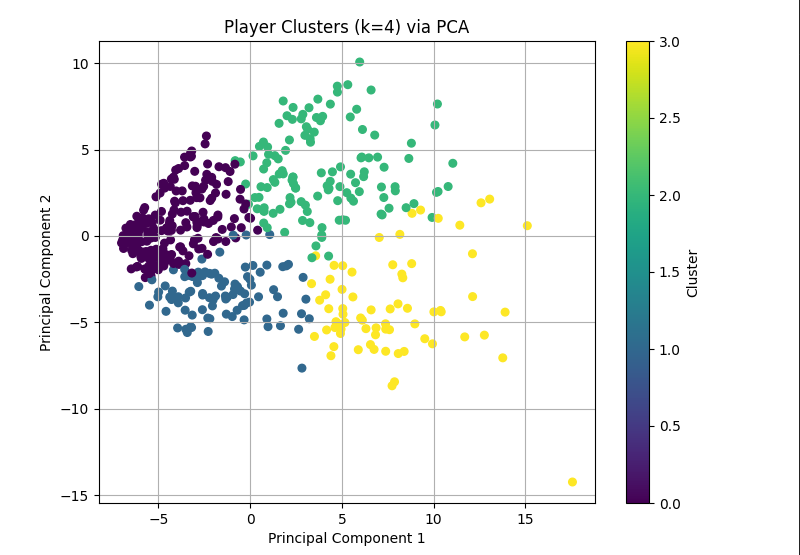
\includegraphics[width=1\textwidth]{k=4.PNG}

\textbf{h) Conclusion} \\
The K-means clustering algorithm, combined with PCA for dimensionality reduction, provides an effective way to group football players based on their performance statistics. The 2D visualization of the clusters offers a clear representation of how players from different positions and playing styles are grouped. This methodology not only aids in understanding player roles but also provides a foundation for further analysis of player performance across different metrics.

The results can be used to identify patterns in player performance, highlight strengths and weaknesses within specific clusters, and inform strategies for team composition based on player characteristics.

\newpage
%_______Kết luận________
\section*{\textcolor{blue}{\Large 5. Conclusion}}
\titleformat{\section}
  {\bfseries\Large}
  {\thesection.}{1em}{}

\setlist[itemize]{noitemsep, topsep=0pt}

\textbf{a) Overview of K-means Clustering} \\
This project systematically analyzed football player performance data to assess team efficiency, categorize player roles, and predict market values using machine learning techniques. By leveraging methods such as data preprocessing, K-means clustering, PCA, and Random Forest Regression, we constructed a comprehensive pipeline that connects performance statistics with role classification and economic evaluation. Visualization techniques were used to enhance the interpretability of the results, ultimately offering deeper insights into the key factors influencing a player’s market value.

\textbf{b) Overview of K-means Clustering} \\
Throughout the execution of the project, we gained valuable hands-on experience in various domains of data science and football analytics. Key learning outcomes include:
\begin{itemize}
    \item Gaining proficiency in collecting and extracting data from online sources.
    \item Cleaning and standardizing real-world sports data for analysis.
    \item Applying clustering methods to discover natural groupings of players based on performance.
    \item Using regression models to predict target outcomes, such as player market value.
    \item Employing PCA and visualization techniques to better interpret complex data.
    \item Drawing meaningful conclusions from statistical patterns within the football context.
\end{itemize}

\textbf{c) Future Improvements} \\
Despite the effectiveness of the current approach, several directions can be pursued to enhance the model’s utility and performance:
\begin{itemize}
    \item Expanding the dataset to include more seasons, leagues, and player samples to improve model robustness and generalizability.
    \item Integrating contextual features such as injuries, match time, or team economic data for a more holistic analysis.
    \item Experimenting with advanced regression techniques like XGBoost or deep learning models to increase prediction accuracy.
    \item Developing an interactive dashboard to allow stakeholders to dynamically explore player statistics and cluster insights.
\end{itemize}
Overall, this work contributes a solid base for data-driven decision-making in modern football, supporting talent identification, performance evaluation, and market valuation strategies.

\end{document}
